%This is the first chapter of the dissertation

%The following command starts your chapter. If you want different titles used in your ToC and at the top of the page throughout the chapter, you can specify those values here. Since Columbia doesn't want extra information in the headers and footers, the "Top of Page Title" value won't actually appear.

\chapter[A search for supersymmetric particles in zero lepton final states with the Recursive Jigsaw Technique][Top of Page Title]{Title of Chapter 1}

This section presents the details of the first search employing RJR variables as discriminating variables, as described in \ref{ATLAS-CONF-2016-078}.
We will describe the data and simulation samples used, and then define the selections where we search for new SUSY phenomena, which we call the \textit{signal regions} (SRs)
Afterwards, we describe the background estimation techniques used in the analysis.
Finally, we discuss the treatment of systematic uncertainties, and how we combine them using a likelihood method\cite{Baak:2014wma}.

\section{Collision data and simulation samples}

Simulated data is fundamentally important to the ATLAS physics program.
Calibrations, measurements, and searches use Monte Carlo (MC) simulations\footnotemark to compare with collision data.
\footnotetext{In jargon, often just called ``Monte Carlo'' or MC.}
In this thesis, MC samples are used to optimize the signal region selections, assist in background estimation, and assess the sensitivity to specific SUSY signal models.
The details of Monte Carlo production, accuracy, and utility are far beyond the scope of this thesis, but we provide a short description here.

The first step is MC \textit{generation}.
A program is run which does a matrix-element calculation, sometimes with additional corrections, which produces a set of output particles from the parton interactions.
These output particles are then decayed via another (or the same) simulation program.
This produces a set of \textit{truth} particles, which are the output of event generation.
The details of which generator to use are the subject of much discussion, and generally (many) comparisons are made between them, for different processes of interest.
Additionally, differences between generators are often a starting point for the calculation of systematic uncertainties.

The next step is the \textit{simulation}.
The detector response to the truth particles is simulated, and simulated hits are produced.
After simulation, the standard reconstruction algorithms described previously are run with the simulated hits.
This procedure ensures ``as close as possible'' treatment of simulation and collision data.

We give a brief description of which samples use which generators; additional details are available in \ref{ATLAS-CONF-2016-078}.

\todo{MAKE BETTER}
Signal (digluino and disquark) samples are generated with up to two extra partons in the matrix element using MG5\_aMC@NLO~2.2.2 event generator~\cite{Alwall:2014hca} interfaced to  \pythia~8.186~\cite{Sjostrand:2014zea}.
The nominal cross-section is taken from an envelope of cross-section predictions using different PDF sets and factorization and renormalization scales, as described in Ref.~\cite{Kramer:2012bx}, considering only light-flavour quarks ($u$, $d$, $s$, $c$).
For the light-flavour squarks (gluinos) in case of gluino- (squark-) pair production, cross-sections are evaluated assuming masses of 450 \TeV.
The free parameters are $m_{\lsp}$ and $m_{\gluino}$ ($m_{\squark}$) for gluino-pair (squark-pair) production models.
\todo{explain we have a ``grid'' of these signal models samples}
%The {\textsc EvtGen}~v1.2.0 program~\cite{evtgen} is used to describe the properties of the $b$- and $c$- hadron decays in the signal samples, and the background samples except those produced with \sherpa~\cite{sherpa2}.

Boson ($W$, $Z$, $\gamma$) plus jet events are simulated using different \sherpa generators, with \textsc{Comix} and \textsc{OpenLoops} matrix-element generators\cite{ATL-PHYS-PUB-2016-003, comix, openloops}.
Photons are required to have transverse momentum of $> 35 \GeV$.
Importantly, the $W (Z)$+jet events are calculated at NLO while the the $\gamma$+jet events are calculated at LO.
% The production of $W$ or $Z$ bosons in association with jets~\cite{ATL-PHYS-PUB-2016-003} is simulated using the \sherpa~2.2.0 generator, while the production of $\gamma$ in association with jets is simulated using the \sherpa~2.1.1 generator.
%In events with $W$ or $Z$ bosons, the matrix elements calculated using the , and merged with the \sherpa\ parton shower \cite{sherpashower} using the ME+PS@NLO prescription \cite{mepsnlo}. %To fix the scale setting problem, a reweighting procedure based on the number truth jets is applied.
% The samples are produced with a simplified scale setting prescription in the multi-parton matrix elements, to improve the event generation speed. A theory-based re-weighting of the jet multiplicity distribution is applied at event level, derived from event generation with the strict scale prescription.
% Events containing a photon in association with jets are generated requiring a photon transverse momentum above 35~\GeV.
%  For these events, matrix elements are calculated at LO with up to three or four partons depending on the $\pt$ of the photon, and merged with the \sherpa\ parton shower using the ME+PS@LO prescription~\cite{Hoeche:2009rj}.
%In the case of $W/Z$+jets, the NNPDF3.0NNLO PDF set \cite{Ball:2014uwa} is used, while for the $\gamma$+jets production the CT10 PDF set \cite{CT10pdf} is used, both in conjunction with dedicated parton shower-tuning developed by the authors of \sherpa.
The $W/Z$ + jets events are normalized to their NNLO cross-sections \cite{Catani:2009sm}.
The $\gamma$+jets LO cross-section is taken directly from \sherpa; we will apply a correction factor to be described later.\todo{THISSSSSS}

The various \ttbar and single-top processes\cite{ATL-PHYS-PUB-2016-004} are generated using two versions of \textsc{Powheg-Box} \cite{ATL-PHYS-PUB-2016-004,powheg-box}.
These are calculated at NLO and normalized to various orders ranging from NLO to NNLO+NNLL in the different processes, which can be seen in \ref{tab:montecarlo}\cite{Czakon:2013goa,Czakon:2011xx,Aliev:2010zk,Kant:2014oha,Kidonakis:2010ux,Kidonakis:2011wy}.
% For the generation of $t\bar{t}$ and single-top processes in the $Wt$ and $s$-channel~\cite{ATL-PHYS-PUB-2016-004}, the \textsc{Powheg-Box} v2 \cite{powheg-box} generator is used with the CT10 PDF set.
% The electroweak (EW) $t$-channel single-top events are generated using the \textsc{Powheg-Box} v1 generator.
% This generator uses the four-flavour scheme for the NLO matrix-element calculations together with the fixed four-flavour PDF set CT10f4~\cite{CT10pdf}.
% For this process, the decay of the top quark is simulated using {\textsc MadSpin} tool \cite{10a} preserving all spin correlations, while for all processes the parton shower, fragmentation, and the underlying event are generated using \pythia~6.428 \cite{pythia6} with the CTEQ6L1 \cite{Pumplin:2002vw} PDF set and the corresponding {\textsc Perugia 2012} tune (P2012) \cite{perugia}. The top quark mass is set to 172.5~\GeV.
% The $h_{\rm damp}$ parameter, which controls the $\pt$ of the first additional emission beyond the Born configuration, is set to the mass of the top quark. The main effect of this is to regulate the high-$\pt$ emission against which the ttbar system recoils \cite{ATL-PHYS-PUB-2016-004}.
%The EvtGen v1.2.0 program \cite{evtgen} is used for properties of the bottom and charm hadron decays.
% The $t\bar{t}$ events are normalized to the NNLO+NNLL ~\cite{Czakon:2013goa,Czakon:2011xx}.
% The $s$- and $t$-channel single-top events are normalized to the NLO cross-sections \cite{}, and the $Wt$-channel single-top events are normalized to the NNLO+NNLL~\cite{}.
% For the generation of $t\bar{t}$ + EW processes ($t\bar{t} + W/Z/WW$)~\cite{ATL-PHYS-PUB-2016-005}, the MG5\_aMC@NLO~2.2.3~\cite{Alwall:2014hca} generator at LO interfaced to the \pythia~8.186 parton-shower model is used, with up to two ($t\bar{t}+W$, $t\bar{t}+Z(\to \nu\nu/qq)$), one ($t\bar{t}+Z(\to \ell\ell)$) or no ($t\bar{t}+WW$) extra partons included in the matrix element.
% The ATLAS underlying-event tune A14 is used together with the NNPDF2.3LO PDF set.
% The events are normalized to their respective NLO cross-sections~\cite{Lazopoulos:2008de,Campbell:2012dh}.

Diboson processes ($WW$, $WZ$, $ZZ$)~\cite{ATL-PHYS-PUB-2016-002} are simulated using the  \sherpa~2.1.1 generator
For processes with four charged leptons (4$\ell$), three charged leptons and a neutrino (3$\ell$+1$\nu$) or two charged leptons and two neutrinos (2$\ell$+2$\nu$), the matrix elements contain all diagrams with four electroweak vertices, and are calculated for up to one (4$\ell$, 2$\ell$+2$\nu$) or no partons (3$\ell$+1$\nu$) at NLO and up to three partons at LO using the \textsc{Comix} and \textsc{OpenLoops} matrix-element generators, and merged with the \sherpa\ parton shower using the ME+PS@NLO prescription.
For processes in which one of the bosons decays hadronically and the other leptonically, matrix elements are calculated for up to one ($ZZ$) or no ($WW$, $WZ$) additional partons at NLO and for up to three additional partons at LO using the \textsc{Comix} and \textsc{OpenLoops} matrix-element generators, and merged with the \sherpa\ parton shower using the ME+PS@NLO prescription.
In all cases, the CT10 PDF set is used in conjunction with a dedicated parton-shower tuning developed by the authors of  \sherpa.
The generator cross-sections are used in this case.

The multi-jet background is generated with \pythia~8.186 using the A14 underlying-event tune and the NNPDF2.3LO parton distribution functions.

A summary of the SM background processes together with the MC generators, cross-section calculation orders in $\alpha_{\textrm s}$, PDFs, parton shower and tunes used is given in Table~\ref{tab:montecarlo}.

\begin{table}[H]
\resizebox{\textwidth}{!}{
\begin{tabular}{| l l c c c c |}
\hline
Physics process & Generator& Cross-section & PDF set & Parton shower & Tune \\
&& normalization & & & \\
\hline
$W(\rightarrow \ell\nu)$ + jets              & \sherpa~2.2.0        & NNLO  &  NNPDF3.0NNLO   &  \sherpa\     & \sherpa~default \\
$Z/\gamma^{*}(\rightarrow \ell \bar \ell)$ + jets & \sherpa~2.2.0         & NNLO  &  NNPDF3.0NNLO   & \sherpa\      & \sherpa~default\\
$\gamma $ + jets & \sherpa~2.1.1         & LO  &    CT10  & \sherpa\   & \sherpa~default\\

$t\bar{t}$              & {\textsc Powheg-Box}~v2   & NNLO+NNLL                   &  CT10 &  \pythia~6.428  &\textsc{Perugia2012} \\

%%Single-top              &&&&\\
Single top ($Wt$-channel) & {\textsc Powheg-Box} v2  &  NNLO+NNLL  &  CT10 &  \pythia~6.428   & \textsc{Perugia2012}\\
Single top ($s$-channel)           & {\textsc Powheg-Box} v2  & NLO  &  CT10 &  \pythia~6.428   & \textsc{Perugia2012}\\
Single top ($t$-channel)           & {\textsc Powheg-Box} v1  & NLO  &  CT10f4 &  \pythia~6.428   & \textsc{Perugia2012}\\

$t\bar{t}+W/Z/WW$       &  MG5\_aMC@NLO~2.2.3  & NLO  & NNPDF2.3LO & \pythia~8.186 & A14    \\

$WW$, $WZ$, $ZZ$    &  \sherpa~2.1.1       & NLO  &  CT10 & \sherpa\   & \sherpa~default \\
Multi-jet    &  \pythia~8.186       & LO  & NNPDF2.3LO & \pythia~8.186   & A14\\

\hline
\end{tabular}
\caption{The Standard Model background Monte Carlo simulation samples used in this thesis.
The generators, the order in $\alpha_{\textrm s}$ of cross-section calculations used for yield normalization, PDF sets, parton showers and tunes used for the underlying event are shown.}
\label{tab:montecarlo}
}
\end{table}




%%% Local Variables:
%%% mode: latex
%%% TeX-master: t
%%% End:


%The summary of processes considered together with the MC generators, cross-section calculations and PDFs used are listed in Table~\ref{tab:montecarlo}.
For all SM background samples the response of the detector to particles is modelled with a full ATLAS detector simulation \cite{:2010wqa} based on \textsc{Geant4} \cite{Agostinelli:2002hh}.
Signal samples are prepared using a fast simulation based on a parameterization of the performance of the ATLAS electromagnetic and hadronic calorimeters \cite{ATLAS:2010bfa} and on \textsc{Geant4} elsewhere.
%, or through a fast simulation using a parameterization of the performance of the ATLAS electromagnetic and hadronic calorimeters \cite{ATLAS:2010bfa} and \textsc{Geant4} elsewhere; the latter applies to  \powheg{}+\pythia{} $t\bar{t}$ samples.

All simulated events are overlaid with multiple $pp$ collisions simulated with the soft QCD processes of \pythia~8.186 using the A2 tune  \cite{A14tune} and the MSTW2008LO parton distribution functions \cite{Martin:2009iq}. The simulations are reweighted to match the distribution of the mean number of interactions observed in data. %It was checked that the effect of such pile-up reweighting is completely negligible.

%The MC samples were generated with an expected pile-up distribution (multiple $pp$ interactions in the same or neighbouring bunch-crossings), but have not been reweighted to match the distribution of the mean number of interactions observed in data. It has been checked that the effect of such pile-up reweighting is completely negligible.

%Differing pile-up (multiple $pp$ interactions in the same or neighbouring bunch-crossings) conditions as a function of the instantaneous luminosity are taken into account by overlaying simulated minimum-bias events (simulated using \pythia~8 with the MSTW2008LO PDF set~\cite{Sherstnev:2007nd} and the A2 tune \cite{ATL-PHYS-PUB-2011-014})  onto the hard-scattering process and reweighting events according to the distribution of the mean number of interactions observed in data.

\section{Event selection}

This section describes the selection of events.
We begin by describing the \textit{preselection}, which is used to remove problematic events and reduce the dataset to a manageable size.
We then describe the signal region strategy, and present the signal regions used in the analysis.

\subsection{Preselection}

The preselection is used to reduce the dataset to that of interest in this thesis.
The table containing the preselection cuts is shown in \ref{tab:preselection}.
This selection is also used for the samples used for background estimation, except for the lepton veto.

The cuts [1] and [4] are a set of cleaning cuts to remove problematic events.
The \textit{Good Runs List} is a centrally-maintained list of data runs which have been determined to be ``good for physics''.
This determination is made by analysis of the various subdetectors, and monitoring of their status.
Event cleaning is used to veto events which could be affected by noncollision background, noise bursts, or cosmic rays.


We require the lowest unprescaled \met trigger for the data run of interest, as described previously, in cut [2].
The lepton veto is applied in cut [5].
These two cuts are only used for the signal region selection.

The rest of the preselection is used for the signal region and background estimation samples.
These cuts are mostly used for the reduction of the dataset to a manageable
Signal models with sensitivity to lower values of these scale variables have been ruled out by previous searches \todo{cite}.
The final cut is on \meff, which is the scalar sum of all jets and \met.
This is the final discriminating variable used in the complementary search to this thesis, which is also presented in \ref{ATLAS-CONF-2016-078}.


\begin{table}[tbp]
  {\small
  \begin{center}\renewcommand\arraystretch{1.4}
   \hspace*{-0.05\textwidth}
   \begin{tabular}{|c|l|c|}
      \hline
      Cut           & Description              & \\
      \hline
      \hline
     1 &Good Runs List& Veto events with intolerable detector errors \\ \hline
     2  & Event cleaning                                            & Veto for noncollision background, noise bursts,  and cosmic rays \\ \hline
     3  & \met [GeV] $>$                                            &  250                                                \\ \hline
     4  & $\pt(j_1)$ [GeV] $>$                                      &  200                                                \\ \hline
     5 & $\pt(j_2)$ [GeV] $>$                                      &   50                                                  \\ \hline
     6 & $\meff$ [GeV] $>$                                         &  800                                                \\ \hline
   \end{tabular}
\caption{\label{tab:preselection} Preselection for the various event topologies used in the analysis.}
  \end{center}
}
\end{table}

%%% Local Variables:
%%% mode: latex
%%% TeX-master: t
%%% End:


\subsection{Signal regions}
We define a set of of signal regions using the RJR variables previously described.
These signal regions are split into three general categories: squark pair production SRs, gluino pair production SRs, and compressed production SRs.
Within these general SRs, we have a set of signal regions targetting different mass splittings of the sparticle and LSP.
\begin{figure}
\caption{Schematic leading the development of the SUSY signal regions in this thesis.
A variant of this schematic is used for most SUSY searches on ATLAS and CMS.
} \label{fig:sr_schematic}
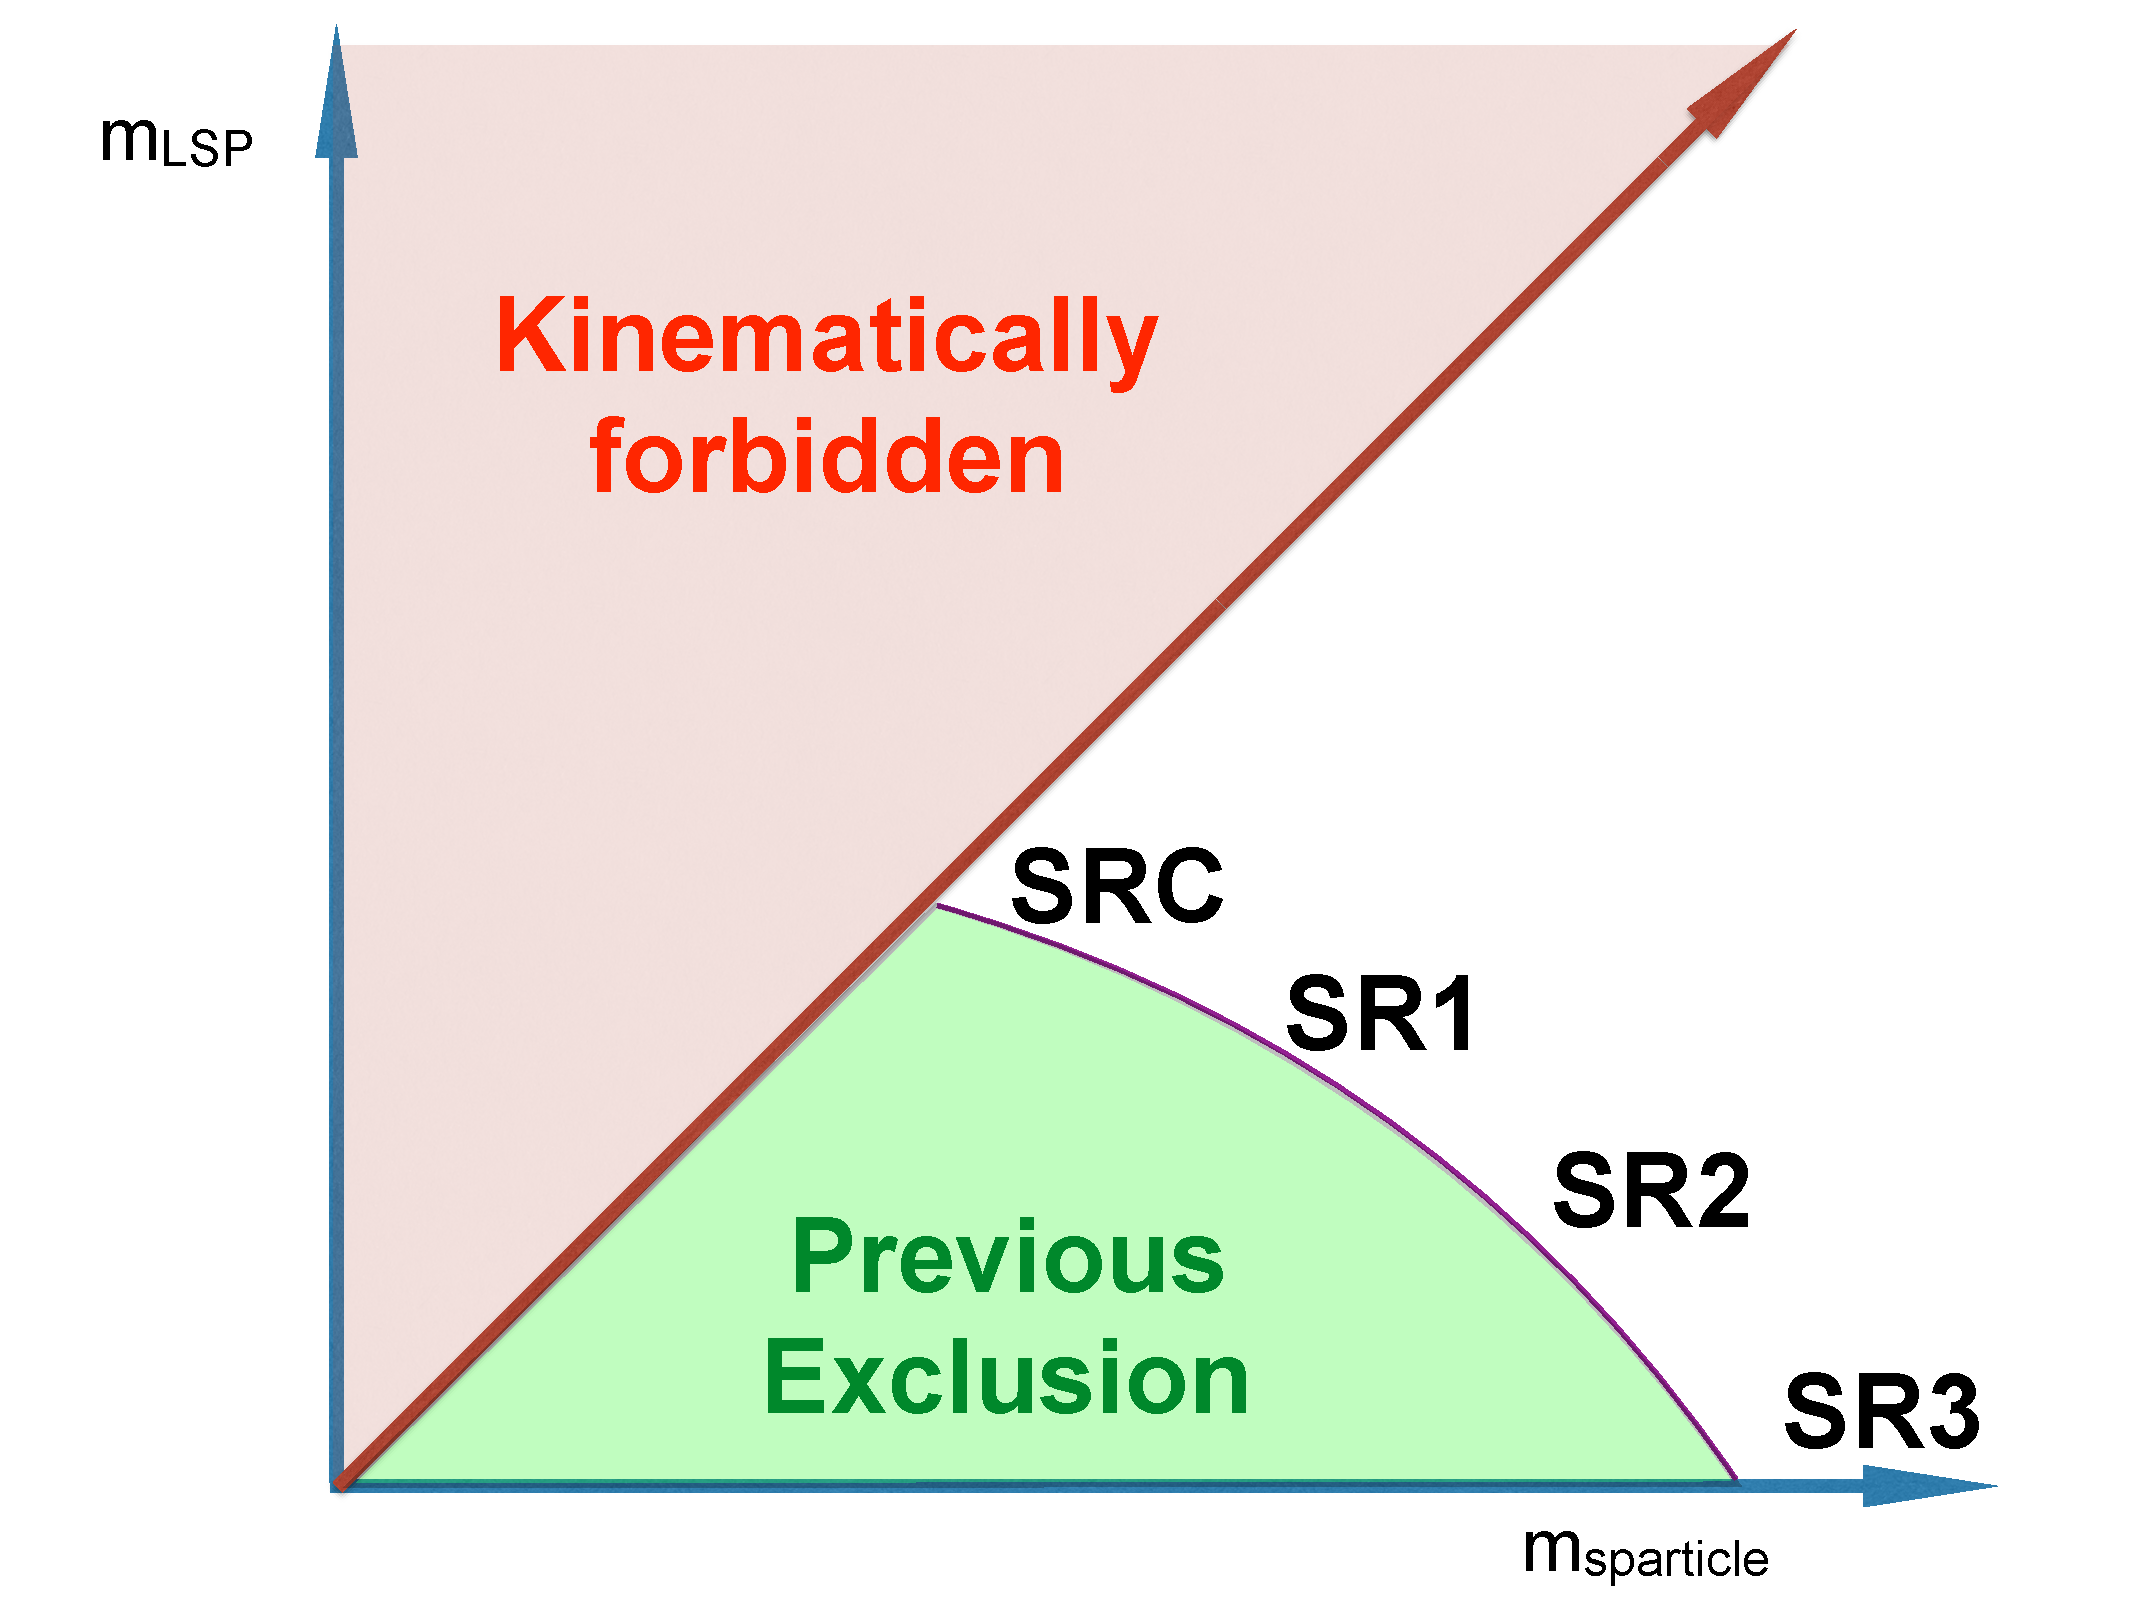
\includegraphics[width=.9\linewidth]{sr_schematic}
\end{figure}

A schematic of this strategy is shown in \ref{sr_schematic}.
This type of plane is how most ($R-$ parity conserving) SUSY searches are organized in both ATLAS and CMS.
The horizontal axis is the mass of the sparticle considered.
In the case of this thesis, this will the squark or gluino mass.
On the horizontal axis, we place the LSP mass.
These are the two free parameters of the simplified models considered here.
Our search occurs in this two-parameter space.
Each signal region targets some portion of this plane.
As shown in the figure, a new iteration of a search will use a set of signal regions which have sensitivity just beyond those of the previous exclusions.
The choice of how many signal regions to use to fully cover this plane is in many ways a matter of judgment, as it is essentially a matter of under/over-fitting to the signal models of interest.
One signal region will obscure the different phenomena in signal events with large versus small mass splittings, leading to underfitting.
Binning as finely as possible\footnotemark leads to overfitting due to the fluctuations present in the signal and background events passing this selection.
\footnotetext{This can be defined as having a signal region for each simulated signal sample, which for this analysis is \order 100.}
In this thesis, we use six squark signal regions, six gluino signal regions, and five compressed regions, which we describe below.

The full table defining all signal regions is shown in \ref{tab:RJsrdefs}.
In all cases, the signal region selections contain a combination of scaleful and scaleless cuts.
Emphasis on cuts on scaleful variables provide stronger sensitivity to larger mass splittings, while additional sensitivity to smaller mass splittings is found using stronger cuts on scaleless variables.
One envisions walking from SR1 (with tight scaleless cuts and loose scaleful cuts) in \ref{fig:sr_schematic} towards SR3 by loosening the scaleless cuts and tightening the scaleful cuts.
We will see this strategy at work in each set of signal regions.

We have already described the useful variables in the previous chapter.
The question is how to choose the optimal cuts for a given set of signal models, which are grouped in the mass splitting space.
This was done by a brute force scan over the cut values, using a guess of integrated luminosity with a fixed systematic uncertainty scenario, motivated by that from previous analyses.
We choose the lowest cut value that maximizes the $Z_{\text{Bi}}$, as described in \cite{Cousins:2008zz}.
This figure of merit gives conservative estimates, as compared to i.e. $S/\sqrt{B}$.
A figure showing an example of this selection tuning procedure is shown in \ref{fig:sr_optimization}.

\begin{figure}
\caption{Optimization of the \HTFnm{PP}{4}{1} cut for a gluino signal model with $(m_{\gluino}, m_{\lsp} ) = (1500,700) \GeV $ assuming 10 \ifb and an uncertainty of 20\% on the background estimate.
} \label{fig:sr_optimization}
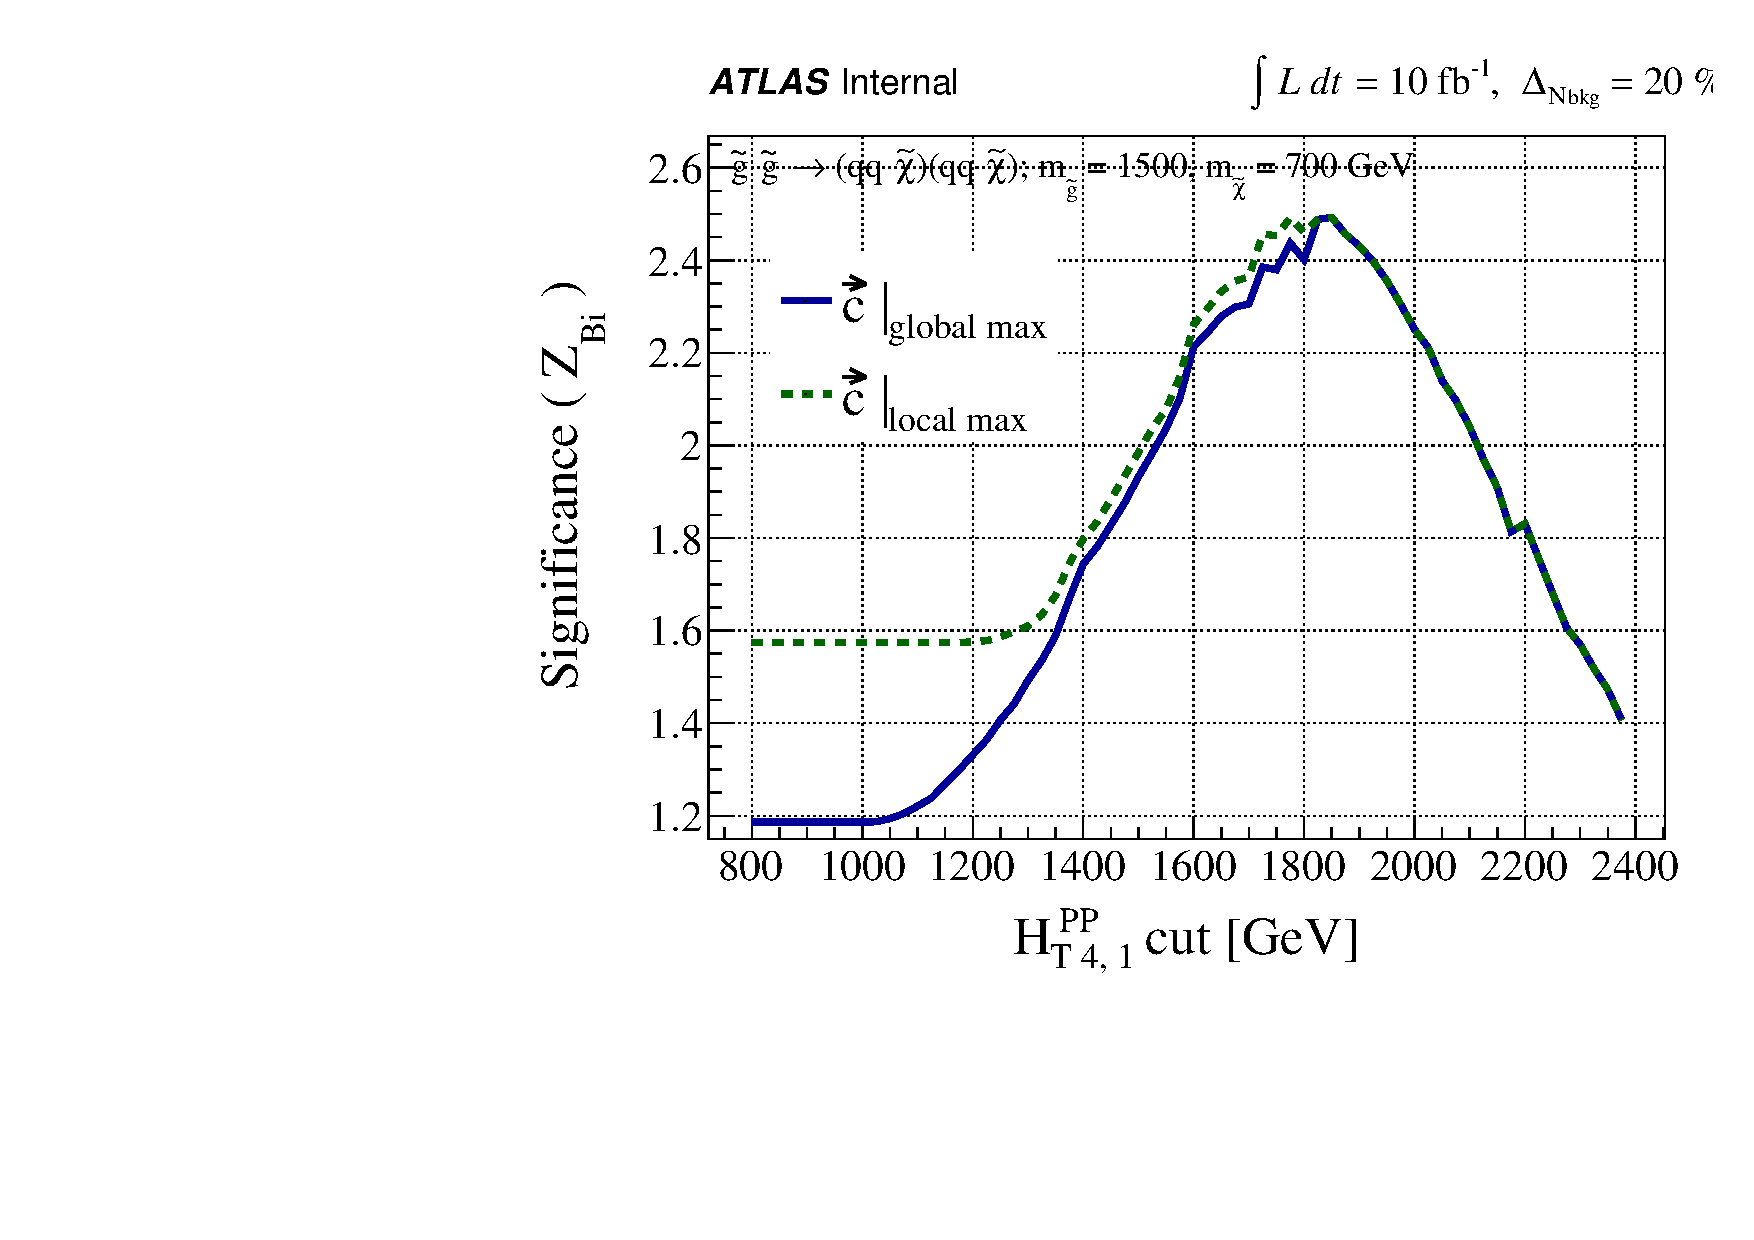
\includegraphics[width=.9\linewidth]{ATLAS-CONF-2016-078_INT/OPT_gluino/HT5PP_10fb_20sys_gg1500_700}
\end{figure}

The compressed selections are split into five regions (SRC1-5), and due to the simplified nature of the compressed decay tree, has sensitivity in both the gluino and squark planes.
The compressed regions target mass splittings with $m_{\text{sparticle}} - m_{\text{LSP}} \tilde{<} 200 \GeV$.
For the compressed region, $M_{T, S}$ is the primary scaleful variable.
We can see the general strategy of lowering increasing scale cuts while decreasing the scaleless cuts here.
SRC1 targets the most compressed scenarios, with mass splittings of less than 25 \GeV, and has the loosest $M_{T, S}$ cut coupled with the tightest \risr and \dphiISR cuts.
SRC4 and SRC5 target mass splittings of $\tilde{~} 200 \GeV$, and are coupled with the loosest scaleless cuts on \risr and \dphiISR.
We also note that SRC4 and SRC5 have differing cuts on \NVjet, since these SRs are closest to the regions we will describe below, and can be see as the ``cross-over'' where the differences between squark and gluino production begins to become manifest.

The squark regions (for noncompressed spectra) are organized into six signal regions.
These are labeled by a numeral 1-3 and letter a/b.
SRs sharing a common numeral i.e. SRS1a and SRS1b share a common set of scaleless cuts, while differing in the main scale variable \HTFnm{PP}{2}{1}.
The two SRs for each set of scaless cuts, only differing in the main scale variable, can be seen in \todo{naive} way as providing sensitivity to a range of luminosity scenarios\footnotemark.
\footnotetext{These SRs were defined before the entire collision dataset was produced, and thus need to be robust in cases where the LHC provides significantly different than expected performance.}
As before, we see that the scaleless cuts are loosened as we tighten the scaleful cuts, as we move across the table from SRS1a to SRS3b.
This provides strong sensivity to signal models with intermediate mass splittings with SRS1a to large mass splittings with SR3b.

The gluino signal regions are organized entirely analogously to the squark signal regions.
There are six gluino signal regions, again labeled via a numeral 1-3 and letter a/b.
Those SRs sharing a common numeral have a common set of scaleless cuts, but differ in their main scale variable \HTFnm{PP}{4}{1}.
The SRs follow the strategy, with SRG1 having the loosest scaleful cut cuts coupled with the strongest scaleless cuts, and the converse being true in SRG3.
As in the squark case, this strategy provides strong expected sensitivity throughout the gluino-LSP plane.
\todo{PLOT expected sensitivity with these assumptions?}

{
\begin{table}[tbp]
\centering
\begin{tabular}{|c|c|c|c|c|c|c|}
\hline
Targeted signal                                                                                                          & \multicolumn{6}{c|}{$\squark\squark$, $\squark \rightarrow q \lsp$}                                                                                              \\
\hline\hline
\multirow{2}{*}{Requirement}                                                                                             & \multicolumn{6}{c|}{Signal Region}                                                                                                                               \\
\cline{2-7}                                                                                                              & \multicolumn{2} {c|}{ \textbf{ S1}} & \multicolumn{2} {c|}{\textbf{S2}} & \multicolumn{2} {c|}{\textbf{S3}}                                        \\
\hline
$H_{\textrm 1,1}^{\textrm ~PP}/H_{\textrm 2,1}^{\textrm ~PP} \geq$                                                       & \multicolumn{2} {c|}{$ 0.6$}            & \multicolumn{2} {c|}{$ 0.55$}          & \multicolumn{2} {c|}{$ 0.5$}                                                  \\ \hline
$H_{\textrm 1,1}^{\textrm ~PP}/H_{\textrm 2,1}^{\textrm ~PP} \leq$                                                       & \multicolumn{2} {c|}{$ 0.95$}           & \multicolumn{2} {c|}{$ 0.96$}          & \multicolumn{2} {c|}{$ 0.98$}                                                 \\ \hline
$p_{\textrm PP,~z}^{\textrm ~lab} / \left( p_{\textrm PP,~z}^{\textrm ~lab}+H_{\textrm T~2,1}^{\textrm ~PP}\right) \leq$ & \multicolumn{2} {c|}{$ 0.5$}            & \multicolumn{2} {c|}{$ 0.55$}          & \multicolumn{2} {c|}{$ 0.6$}                                                  \\ \hline
$p_{\textrm j2,~T}^{\textrm ~PP}/H_{\textrm T~2,1}^{\textrm ~PP} \geq $                                                  & \multicolumn{2} {c|}{$ 0.16$}           & \multicolumn{2} {c|}{$ 0.15$}          & \multicolumn{2} {c|}{$ 0.13$}                                                 \\ \hline
$\Delta_{\textrm  QCD} > $                                                                                               & \multicolumn{6} {c|}{$ 0.001$}                                                                                                                                   \\
\hline\hline
                                                                                                                         & \textbf{S1a}                       & \textbf{ S1b}                      & \textbf{ S2a} & \textbf{ S2b} & \textbf{ S3a} & \textbf{ S3b} \\
\hline
$H_{\textrm T~2,1}^{\textrm ~PP}$ [GeV] $>$                                                                              & 1000                                    & 1200                                   & 1400              & 1600              & 1800              & 2000              \\
\hline
$H_{\textrm 1,1}^{\textrm ~PP}$ [GeV] $>$                                                                                & \multicolumn{2} {c|}{ 1000}             & \multicolumn{2} {c|}{ 1400}            & \multicolumn{2} {c|}{ 1600}                                                   \\
\hline
\end{tabular}
\caption{Event selection for squark signal regions
\label{tab:squark_srs}}
\end{table}

\vspace*{.01\textwidth}

\begin{table}[tbp]
\begin{tabular}{|c|c|c|c|c|c|c|}
\hline
Targeted signal & \multicolumn{6}{c|}{ $\gluino\gluino$, $\gluino \rightarrow q\bar{q} \lsp$} \\
\hline \hline
\multirow{2}{*}{Requirement}                                                                                             & \multicolumn{6}{c|}{Signal Region}                                                                                                                              \\
\cline{2-7}                                                                                                              & \multicolumn{2} {c|}{\textbf{ G1}} & \multicolumn{2} {c|}{\textbf{ G2}} & \multicolumn{2} {c|}{\textbf{ G3}}                                        \\
\hline
$H_{\textrm 1,1}^{\textrm ~PP}/H_{\textrm 4,1}^{\textrm ~PP} \geq$                                                       & \multicolumn{2} {c|}{$ 0.35$}          & \multicolumn{2} {c|}{$ 0.25$}          & \multicolumn{2} {c|}{$ 0.2$}                                                  \\ \hline
$H_{\textrm T~4,1}^{\textrm ~PP}/H_{\textrm 4,1}^{\textrm ~PP} \geq$                                                     & \multicolumn{2} {c|}{$ 0.8$}           & \multicolumn{2} {c|}{$ 0.75$}          & \multicolumn{2} {c|}{$ 0.65$}                                                 \\ \hline
$p_{\textrm PP,~z}^{\textrm ~lab} / \left( p_{\textrm PP,~z}^{\textrm ~lab}+H_{\textrm T~4,1}^{\textrm ~PP}\right) \leq$ & \multicolumn{2} {c|}{$ 0.5$}           & \multicolumn{2} {c|}{$ 0.55$}          & \multicolumn{2} {c|}{$ 0.6$}                                                  \\ \hline
min~$\left( p_{\textrm j2~T~i}^{\textrm ~PP}/H_{\textrm T~2,1~i}^{\textrm ~PP} \right) \geq$                             & \multicolumn{2} {c|}{$ 0.12$}          & \multicolumn{2} {c|}{$ 0.1$}           & \multicolumn{2} {c|}{$ 0.08$}                                                 \\ \hline
max~$\left( H_{\textrm 1,~0}^{\textrm ~Pi}/H_{\textrm 2,~0}^{\textrm Pi} \right) \leq$                                   & \multicolumn{2} {c|}{$ 0.95$}          & \multicolumn{2} {c|}{$ 0.97$}          & \multicolumn{2} {c|}{$ 0.98$}                                                 \\
\hline
$|\frac{2}{3}\Delta\phi_{\textrm V,P}^{\textrm PP} - \frac{1}{3}\cos\theta_{\textrm p} | \leq$                           & \multicolumn{2} {c|}{$ 0.5$}           & \multicolumn{4} {c|}{--}                                                                                               \\ \hline
$\Delta_{\textrm  QCD} > $                                                                                               & \multicolumn{6} {c|}{$ 0 $}                                                                                                                                     \\
\hline \hline
                                            & \textbf{ G1a}             & \textbf{ G1b}             & \textbf{ G2a}             & \textbf{ G2b} & \textbf{ G3a} & \textbf{ G3b} \\
\hline
$H_{\textrm T~4,1}^{\textrm ~PP}$ [GeV] $>$ & 1000                      & 1200                      & 1500                      & 1900 & 2300 & 2800 \\ \hline
$H_{\textrm 1,1}^{\textrm ~PP}$ [GeV] $>$   & \multicolumn{2} {c|}{600}                             & \multicolumn{2} {c|}{800}        & \multicolumn{2} {c|}{900}                   \\ \hline
\end{tabular}
\caption{Event selection for gluino signal regions
\label{tab:gluino_srs}}
\end{table}

\vspace*{.01\textwidth}

\begin{table}[tbp]
\begin{tabular}{|c|c|c|c|c|c|}
\hline
       Targeted signal & \multicolumn{5}{c|}{ compressed spectra } \\
       \hline \hline
      \multirow{2}{*}{Requirement}                                             & \multicolumn{5}{c|}{Signal Region}                                                           \\
 \cline{2-6}                                                                   & \textbf{ C1} & \textbf{ C2} & \textbf{ C3} & \textbf{ C4} & \textbf{ C5} \\
\hline
$R_{\textrm ISR} \geq $                                                        & $ 0.9$           & $ 0.85$          & $ 0.8$           & $ 0.75$          & $ 0.70$          \\ \hline
$ \Delta\phi_{\textrm ISR,~I} \geq$                                            & $ 3.1$           & $ 3.07$          & $ 2.95$          & $ 2.95$          & $ 2.95$          \\ \hline
$\ourdeltaphishort(\textrm{jet}_{\textrm 1,2},\ourvecptmiss)_{\text{min}} \> $ & -                & -                & -                & 0.4              & 0.4              \\ \hline
$M_{\textrm T S}$ [GeV] $\geq$                                                 & $ 100$           & $ 100$           & $ 200$           & $ 500$           & $ 500$           \\ \hline
$p_{\textrm T S}^{\textrm ~CM}$ [GeV]  $\ge$                                   & $ 800$           & $ 800$           & $ 600$           & $ 600$           & $ 600$           \\ \hline
$N_{\textrm jet}^{\textrm ~V} \geq$                                            & $ 1$             & $ 1$             & $ 2$             & $ 2$             & $ 3$             \\
\hline

\end{tabular}
\caption{Event selection for compressed signal regions
\label{tab:compressed_srs}}
\end{table}
}

%%% Local Variables:
%%% mode: latex
%%% TeX-master: t
%%% End:


\subsection{Scale variable distributions in the signal regions}

In \ref{fig:srs_scale,fig:srg_scale,fig:src_scale}, we can see the distributions of the last scale cut used for each signal region.
These distributions include scale factors derived via the fitting procedure the Standard Model background, which we will describe later in this chapter.
These scale factors are all $\order 1$.
The systematic uncertainties, shown in the banded stripe, are also described later in this section.
Each plot shows the distribution from a signal model which is targetted by the given signal region.

These distributions have all cuts applied except for the cut on this scale variable, which allows us to see the additional discrimination provided by the given variable.
Since signal regions with the same numeral have identical cuts on all cuts other than the main scale variable, we show (a) and (b) on the same figure.
The left-most (right-most) arrow shown is the location of the a (b) cut applied in the analysis.
We call these plot \textit{$N-1$} plots, where $N$ refers to the number of cuts applied in the analysis.
The full set of $N-1$ plots in the signal regions for the other variables used in the analysis are shown in \ref{app:n-1_plots}.
We can see that for the signal models targeted by each signal region, each cut provides unique discrimination against the Standard Model backgrounds.

\todo{captions for these figures}
\begin{figure}[tbp]
\begin{center}
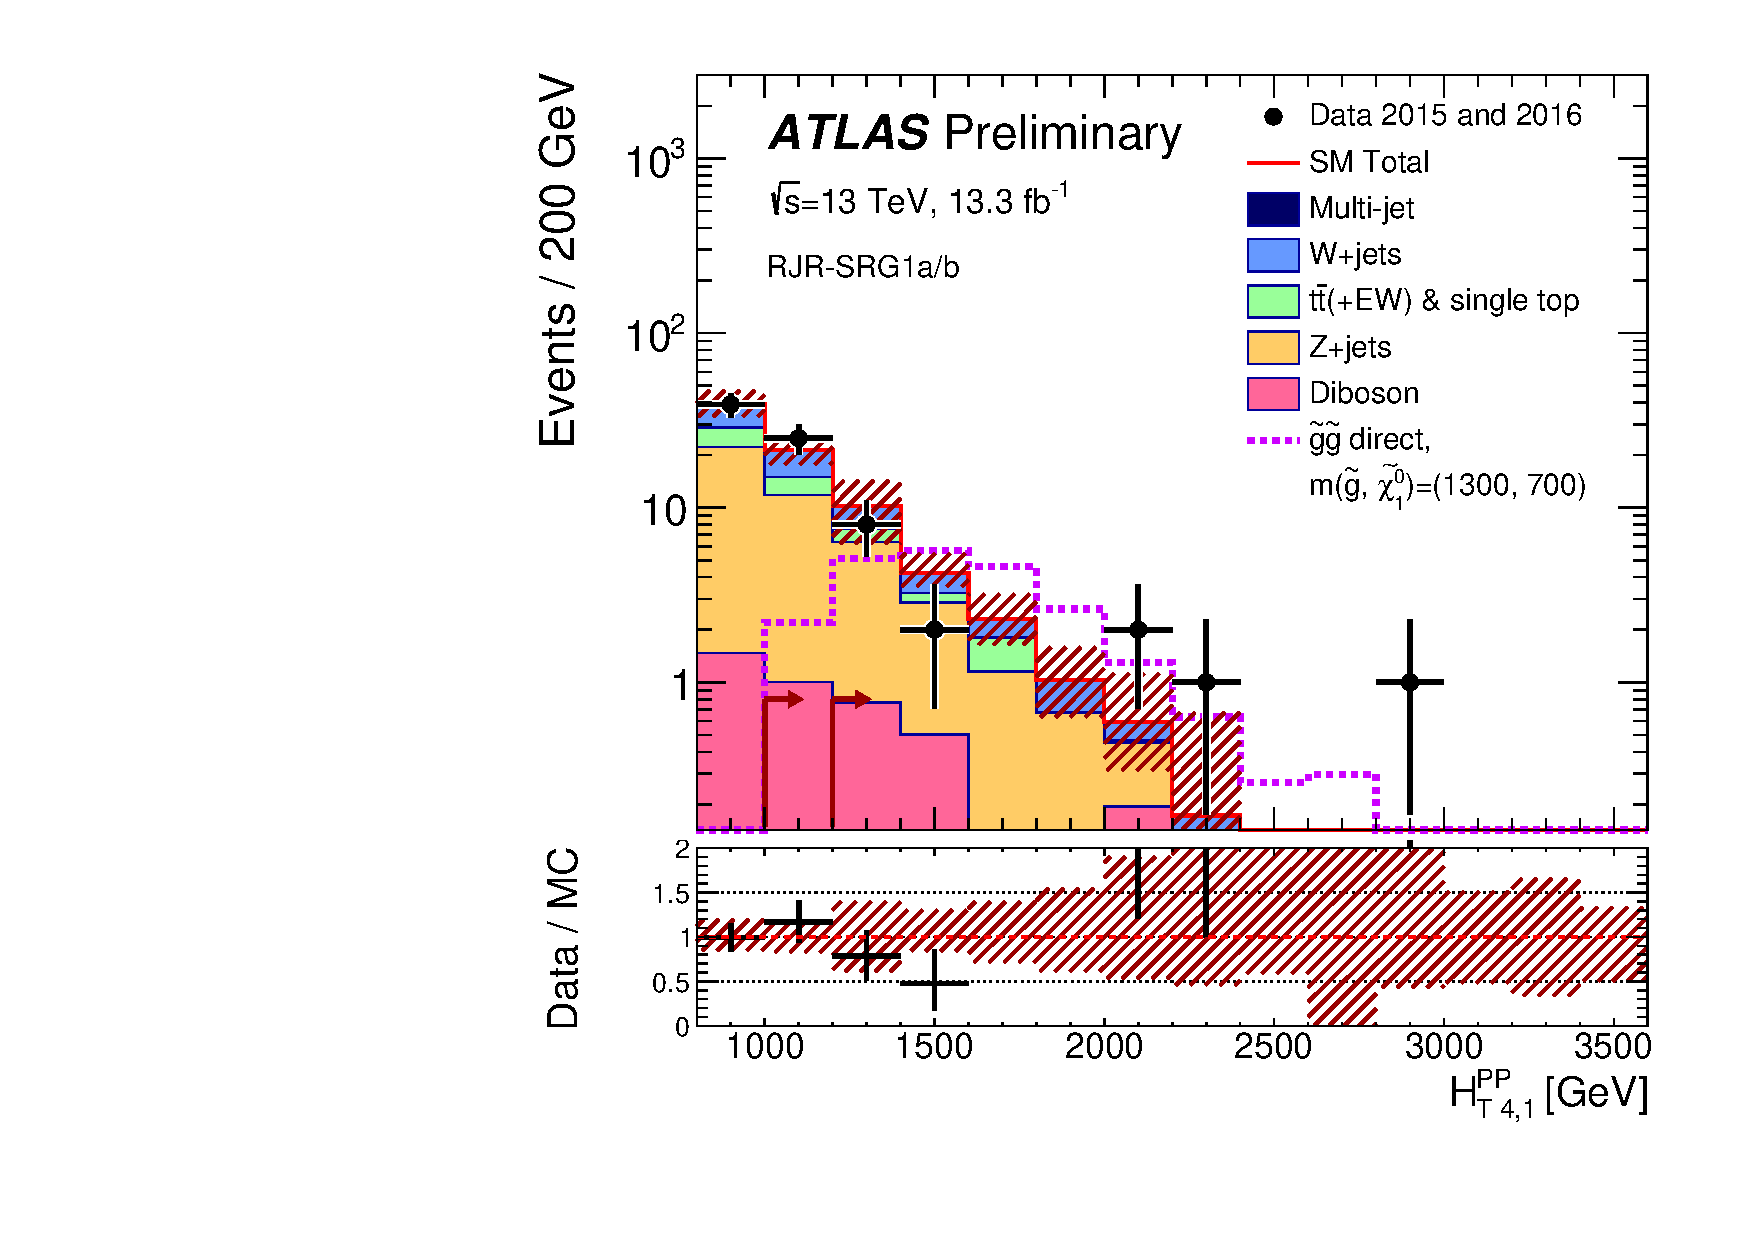
\includegraphics[width=0.45\textwidth]{ATLAS-CONF-2016-078_INT/N-1Plots/AtlasStyle/Preliminary/SR_SRJigsawSRG1a_LastCut_SR_minusone}
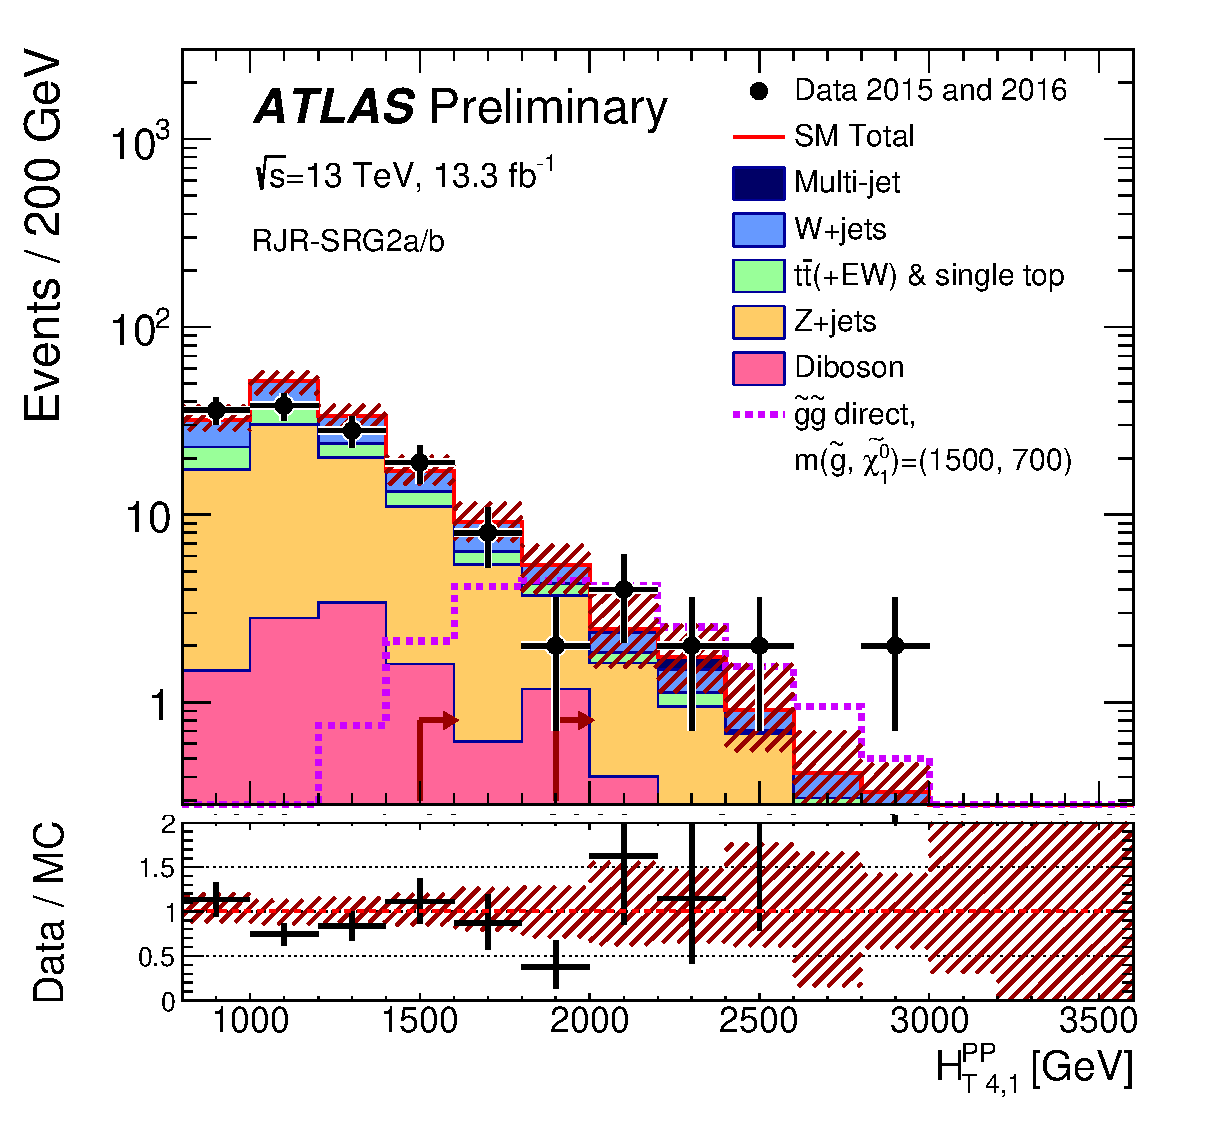
\includegraphics[width=0.45\textwidth]{ATLAS-CONF-2016-078_INT/N-1Plots/AtlasStyle/Preliminary/SR_SRJigsawSRG2a_LastCut_SR_minusone}
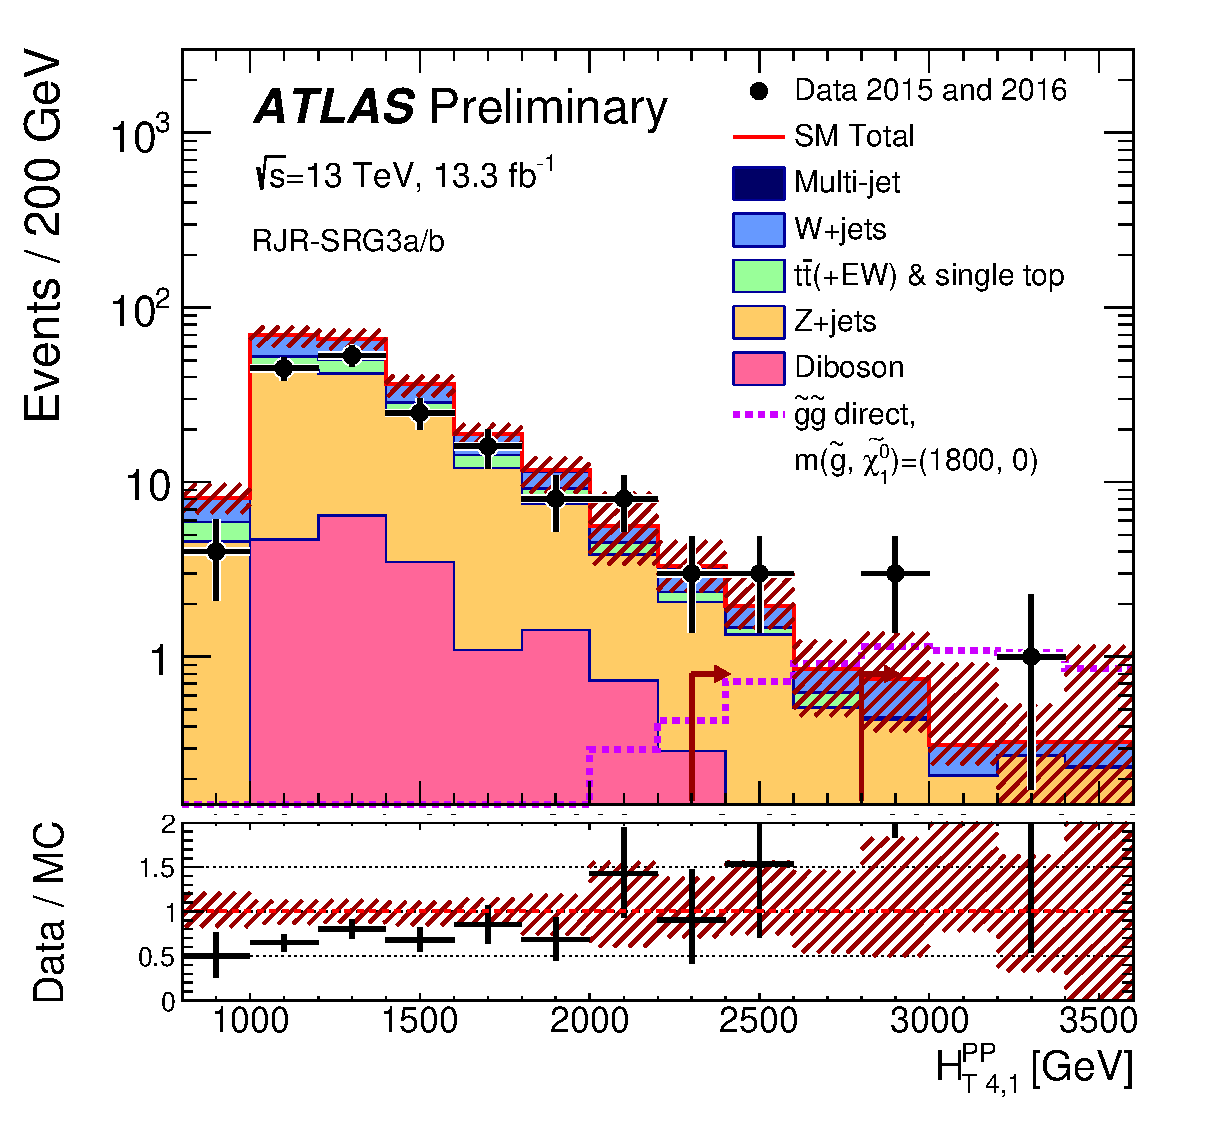
\includegraphics[width=0.45\textwidth]{ATLAS-CONF-2016-078_INT/N-1Plots/AtlasStyle/Preliminary/SR_SRJigsawSRG3a_LastCut_SR_minusone}
\end{center}
\caption{Scale variable distributions for the gluino signal regions.}
\label{fig:srg_scale}
\end{figure}

\begin{figure}[tbp]
\begin{center}
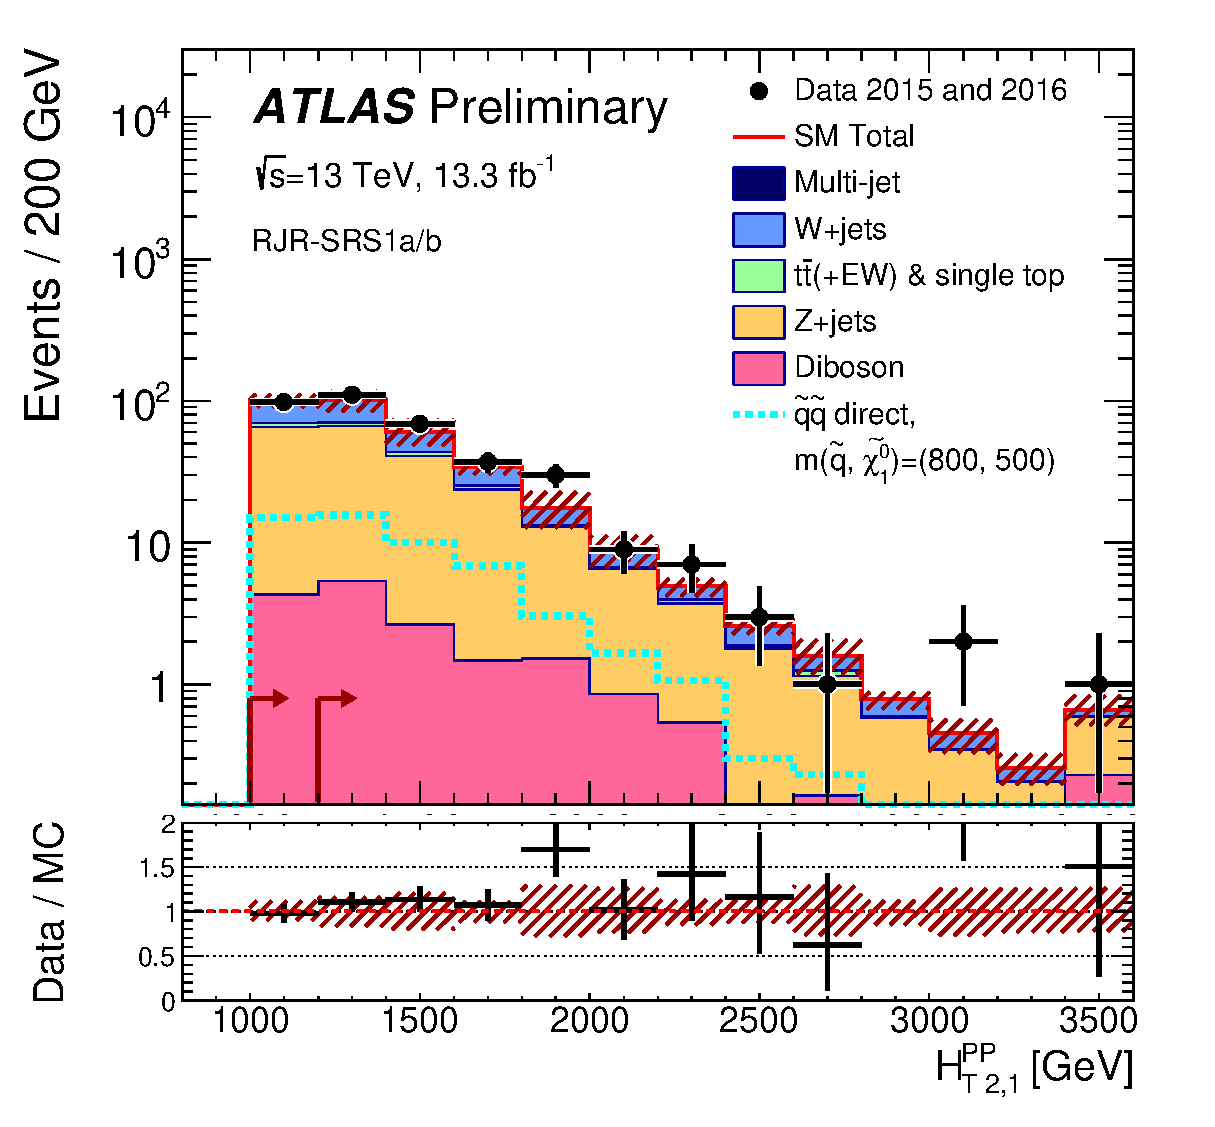
\includegraphics[width=0.45\textwidth]{ATLAS-CONF-2016-078_INT/N-1Plots/AtlasStyle/Preliminary/SR_SRJigsawSRS1a_LastCut_SR_minusone}
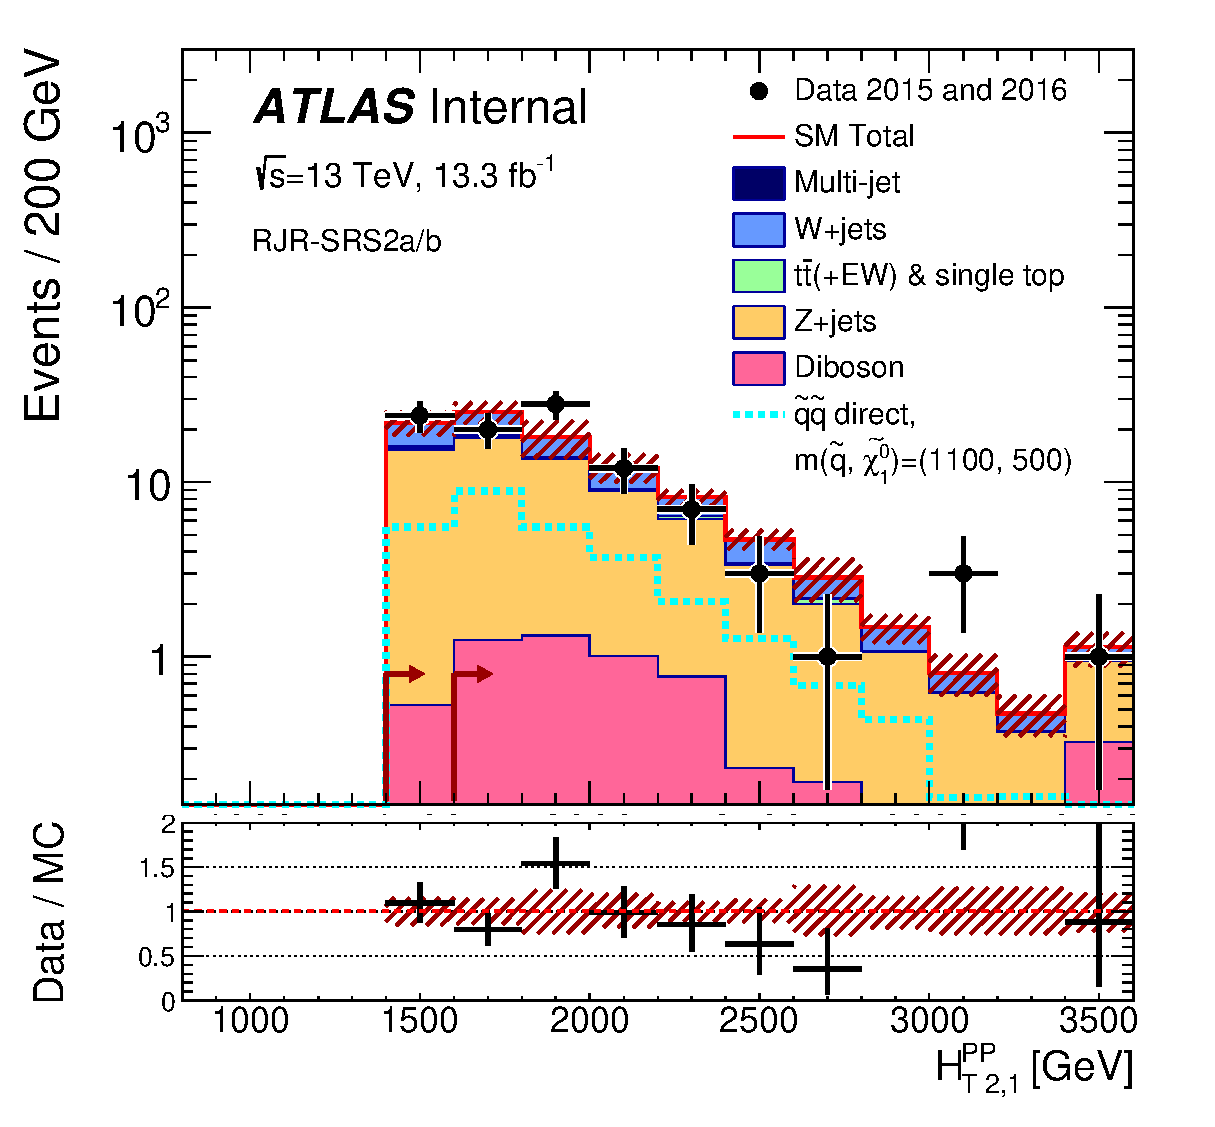
\includegraphics[width=0.45\textwidth]{ATLAS-CONF-2016-078_INT/N-1Plots/AtlasStyle/Preliminary/SR_SRJigsawSRS2a_LastCut_SR_minusone}
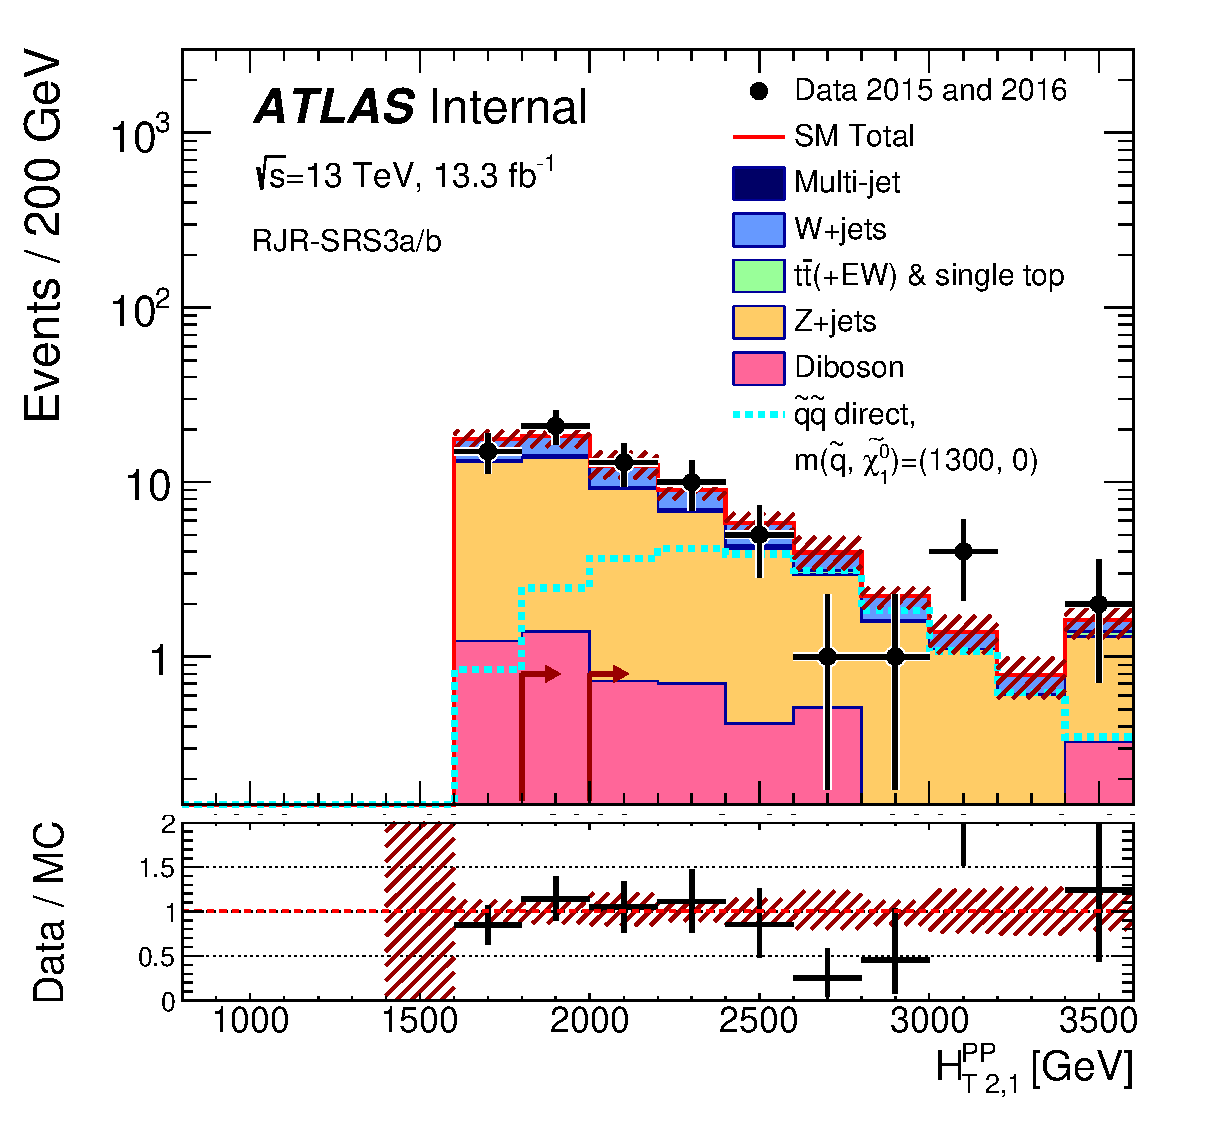
\includegraphics[width=0.45\textwidth]{ATLAS-CONF-2016-078_INT/N-1Plots/AtlasStyle/Preliminary/SR_SRJigsawSRS3a_LastCut_SR_minusone}
\end{center}
\caption{Scale variable distributions for the squark signal regions.}
\label{fig:srs_scale}
\end{figure}

\begin{figure}[tbp]
\begin{center}
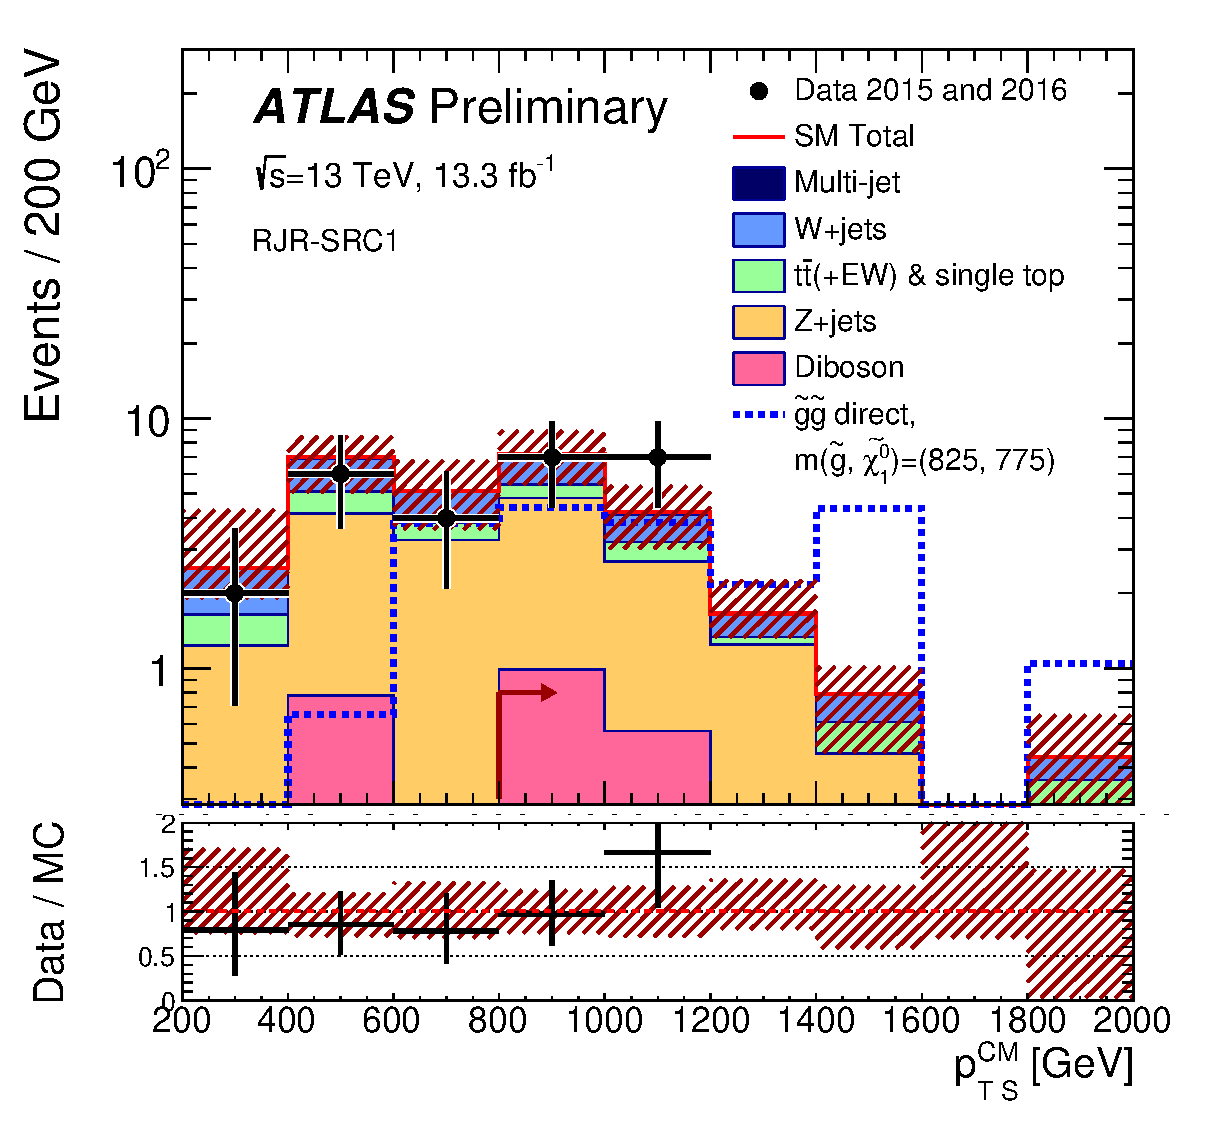
\includegraphics[width=0.45\textwidth]{ATLAS-CONF-2016-078_INT/N-1Plots/AtlasStyle/Preliminary/SR_SRJigsawSRC1_LastCut_SR_minusone}
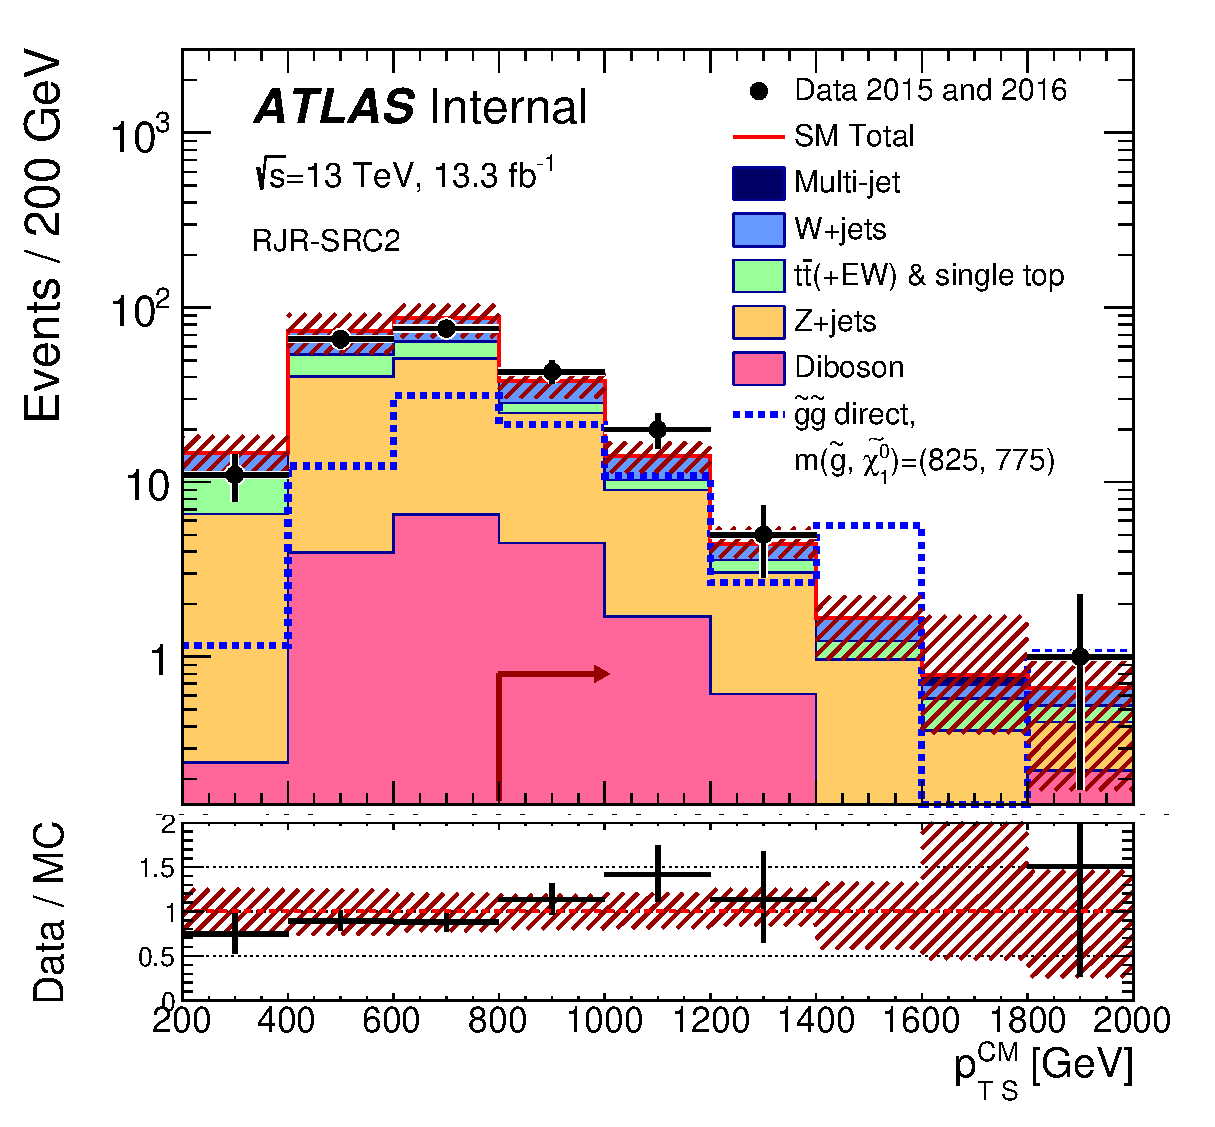
\includegraphics[width=0.45\textwidth]{ATLAS-CONF-2016-078_INT/N-1Plots/AtlasStyle/Preliminary/SR_SRJigsawSRC2_LastCut_SR_minusone}
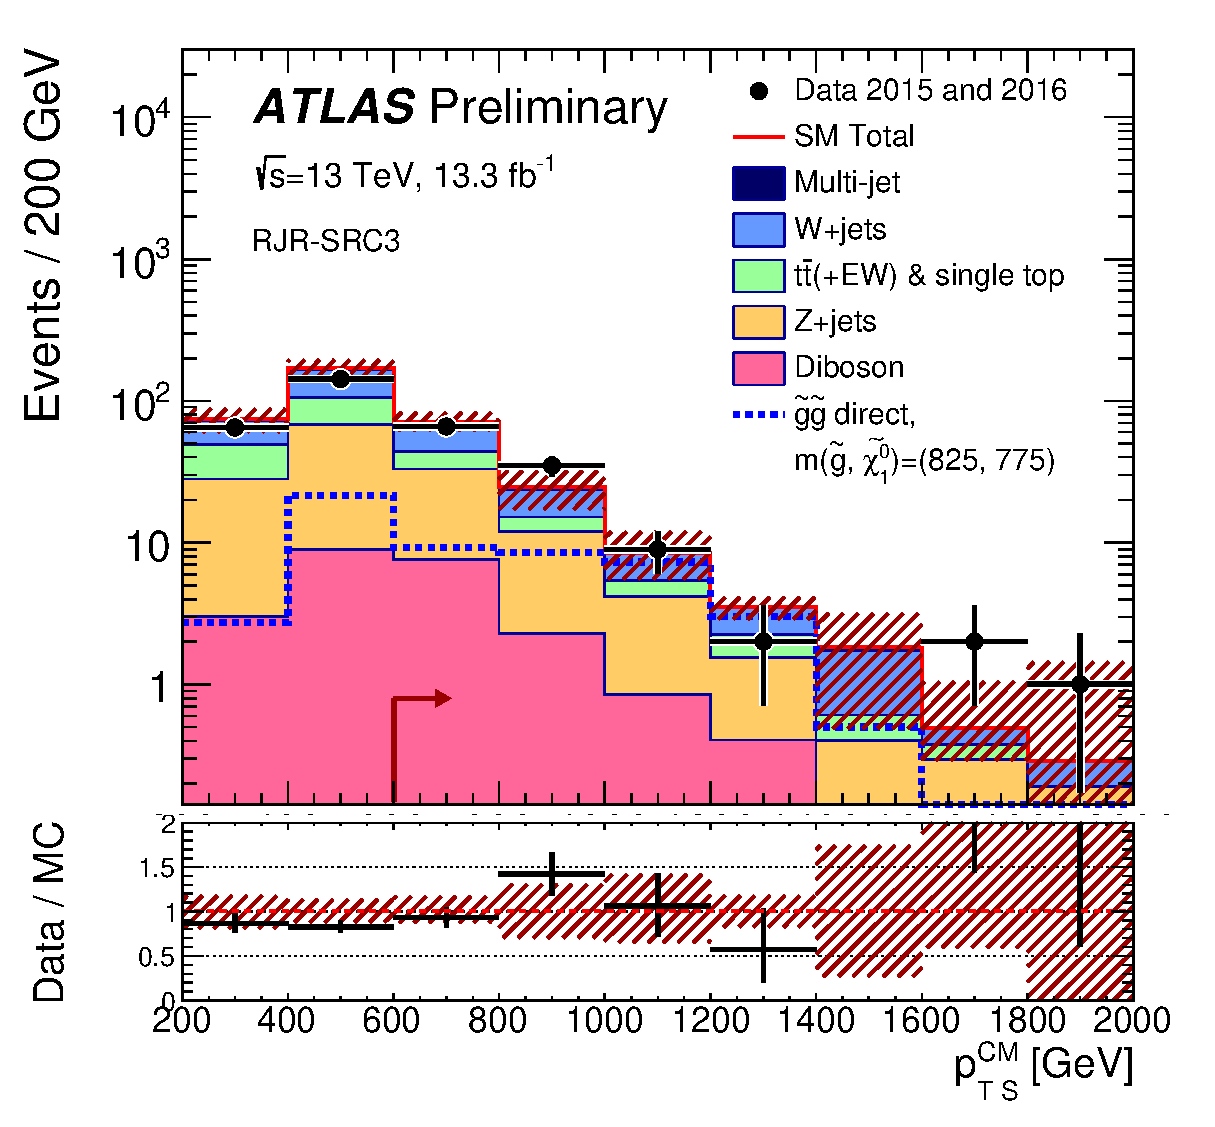
\includegraphics[width=0.45\textwidth]{ATLAS-CONF-2016-078_INT/N-1Plots/AtlasStyle/Preliminary/SR_SRJigsawSRC3_LastCut_SR_minusone}
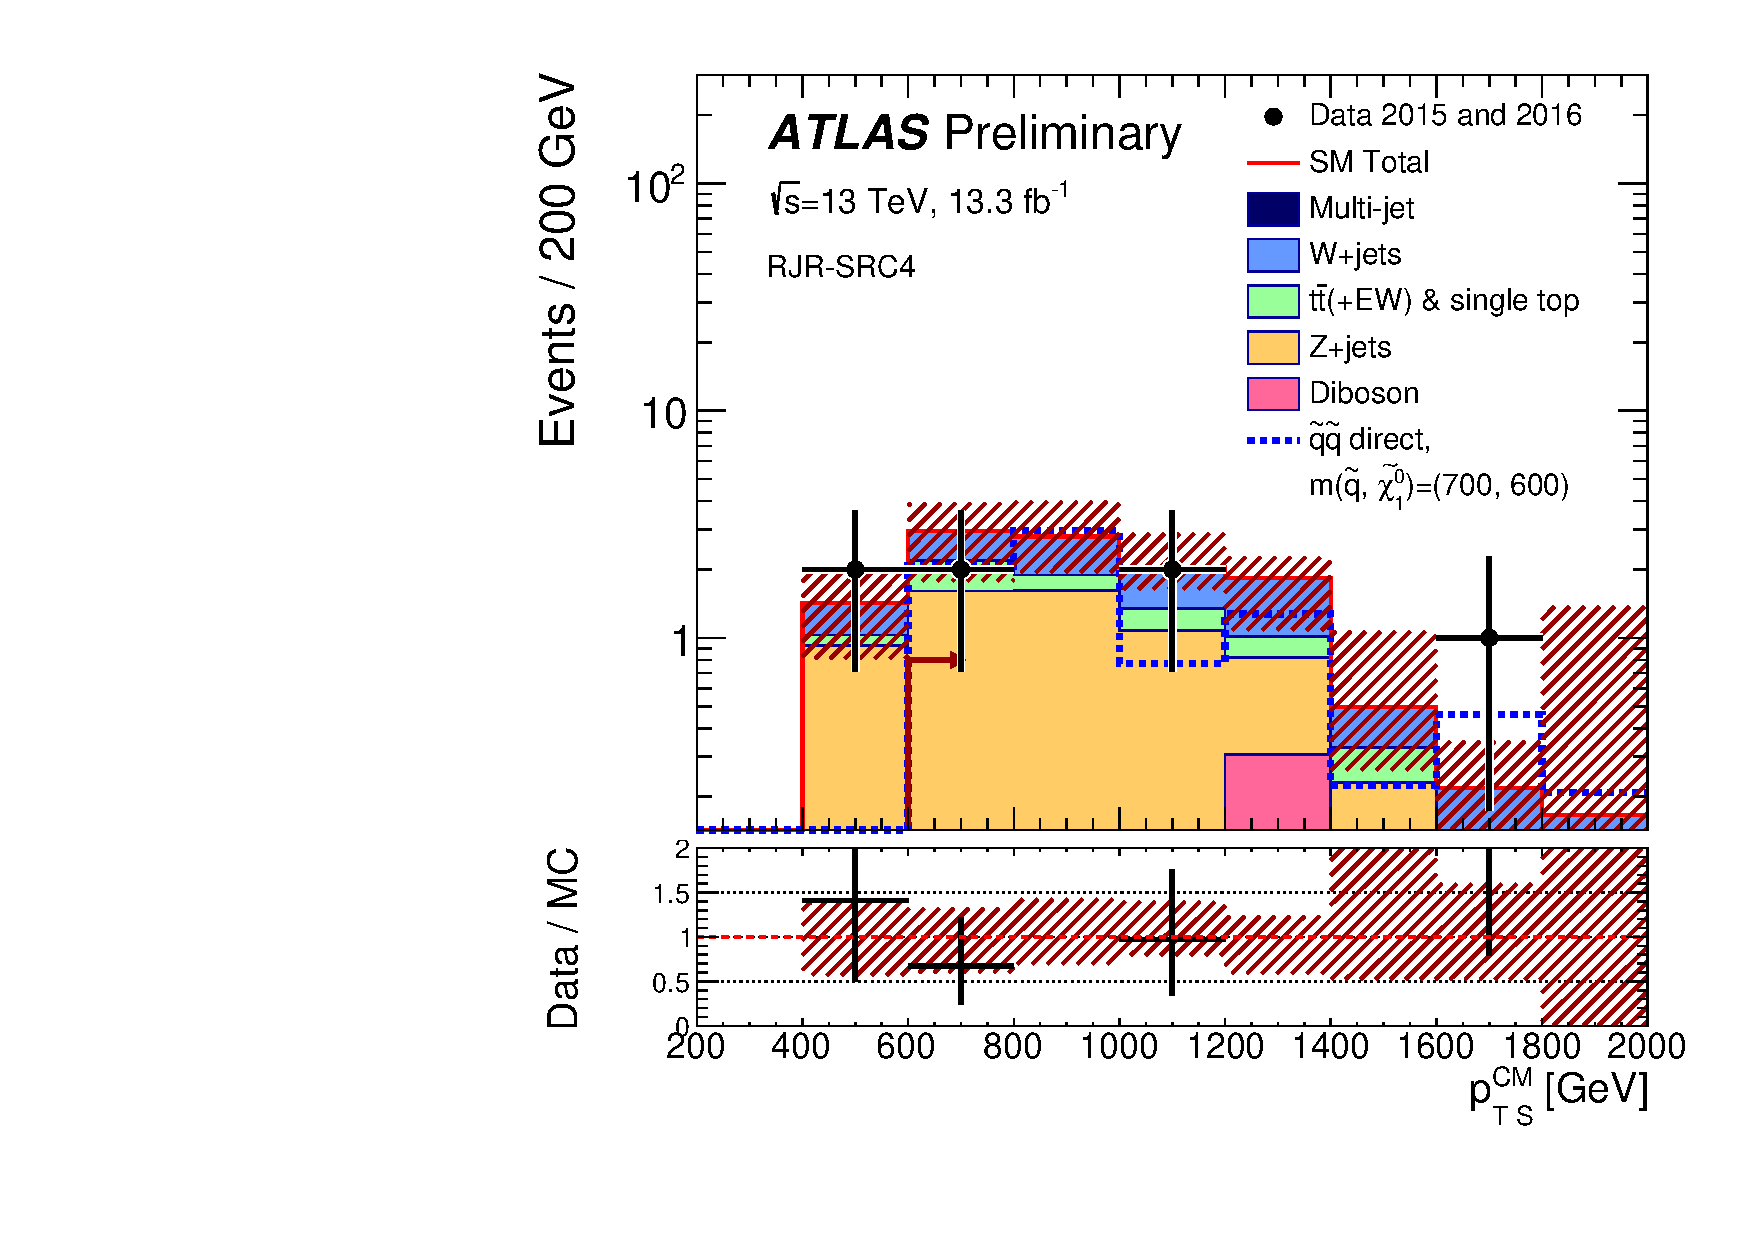
\includegraphics[width=0.45\textwidth]{ATLAS-CONF-2016-078_INT/N-1Plots/AtlasStyle/Preliminary/SR_SRJigsawSRC4_LastCut_SR_minusone}
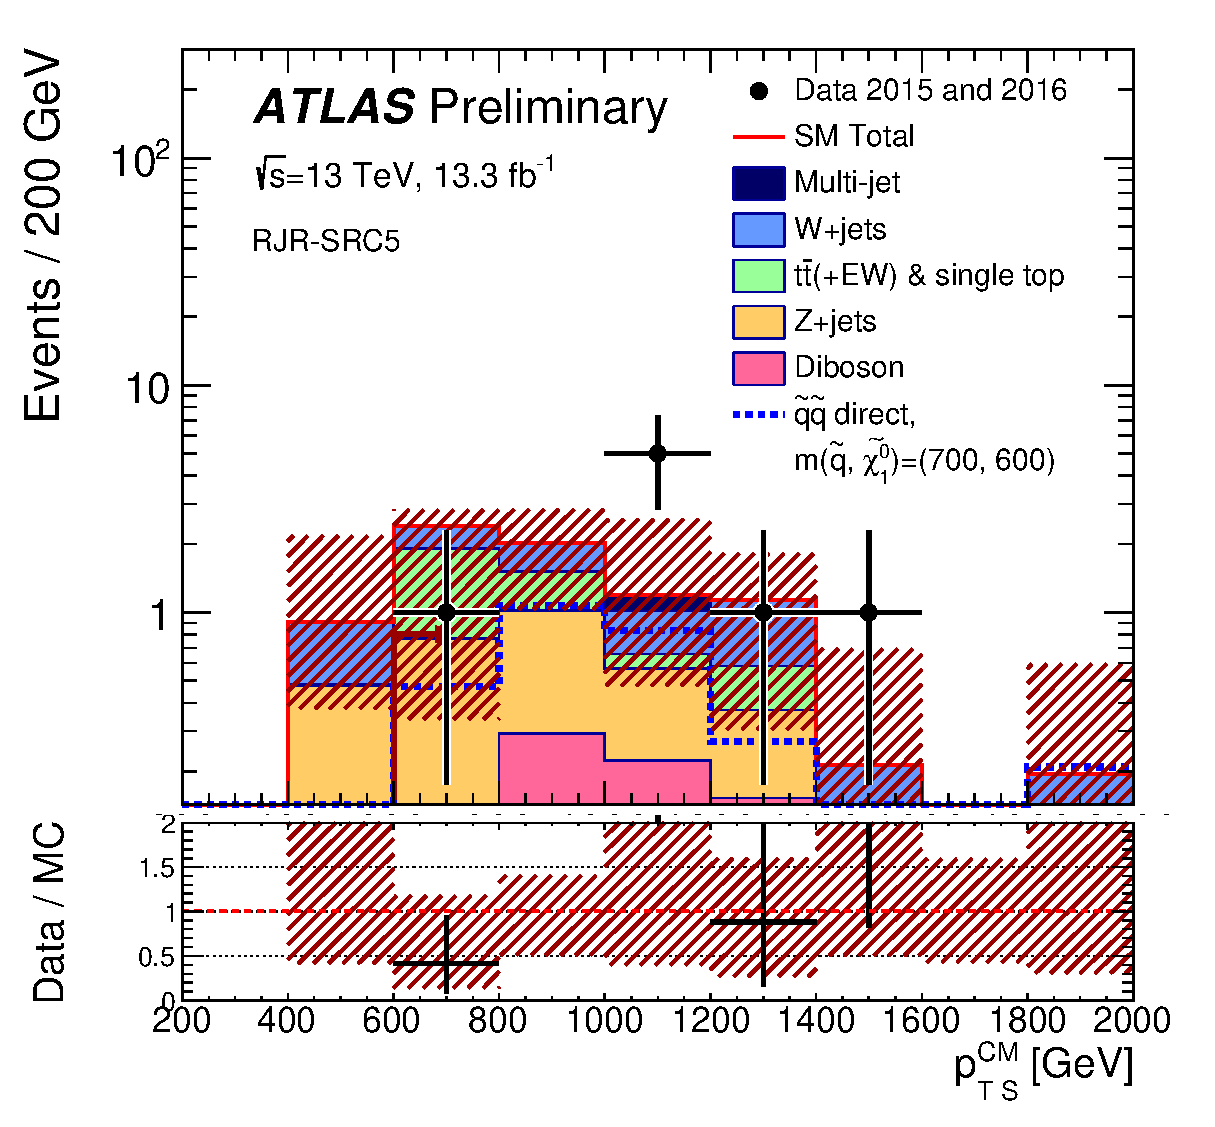
\includegraphics[width=0.45\textwidth]{ATLAS-CONF-2016-078_INT/N-1Plots/AtlasStyle/Preliminary/SR_SRJigsawSRC5_LastCut_SR_minusone}
\end{center}
\caption{Scale variable distributions for the compressed signal regions.}
\label{fig:src_scale}
\end{figure}


\section{Background estimation}

\subsection{Control and Validation Regions}

CRT,CRW,CRY,CRQ

\subsection{R Z/$\gamma$ method}

\subsection{Systematic Uncertainties}
